
\documentclass[12pt]{article}
\usepackage{amsmath}

\usepackage{indentfirst}
%\usepackage[font=small]{caption}10
\usepackage[font=footnotesize]{caption}%9
%\usepackage[font=scriptsize]{caption}%8

\usepackage[utf8]{inputenc}
\usepackage{graphicx}
\usepackage{hyperref}
\usepackage[letterpaper,margin=0.75in]{geometry}
\usepackage{setspace}


\begin{document}

\doublespacing
%\maketitle

\begin{center}
{\Large \textbf{Developments of a Simple Model to Elucidate the Shape of Enveloped Viruses: Motivated by Monkeypox and SARS-CoV-2}}\\[1.5ex]
{\normalsize Student: Hua Deng}\\
{\normalsize Mentor: Dr. Chwen-Yang Shew}\\
{\normalsize February 21, 2025}
\end{center}





\begin{flushleft}
\setlength{\parindent}{45pt}

\section*{Objective}




First, to develop new models and simulations to study how the viral genome architecture(its shape, length and flexibility) influences the membrane. By combining polymer physics and liquid-state physics, such as crowding effects, we hope to gain a deeper understanding of viral assembly. By simulating how viral genomes behave in confined environments, we can uncover key principles behind virus formation and stability. It could contribute to more effective strategies for preventing and treating viral infections, especially for viruses like Monkeypox and SARS-CoV-2.

Second, we into the pressure inside viruses helps us better understand how these tiny organisms infect cells and spread disease. When a virus packages its genetic material into its protein shell, it builds up a lot of internal pressure. This pressure is key to how viruses inject their DNA or RNA into host cells quickly and efficiently. By studying this process, we can uncover new ways to block viruses from replicating, such as targeting the proteins that help pack the genetic material or weakening the capsid so the virus can’t survive. It can inspire new drug delivery systems that work like viruses, help design better and more stable vaccines, and teach us more about the physical limits of DNA and RNA in extreme conditions. In short, understanding viral pressure gives us both the tools to fight disease and ideas to build new technologies.

\section*{Introduction}

Viral infections have a critical impact on global health, emphasizing their role in pandemics and outbreaks. These infections pose significant risks to public health and encompass a wide range of diseases, from seasonal influenza to more severe infectious diseases such as Monkeypox and COVID-19. Both Monkeypox and COVID-19 viruses are classified as enveloped viruses, which are distinguished by their lipid membranes that surround and protect their genetic material (genomes). These membranes serve several crucial functions: they provide protection by shielding the viral genome from environmental factors and potential damage, and they facilitate transmission by enabling the virus to enter host cells. The membrane proteins and polysaccharides play a key role in this process by interacting with specific receptors on host cells, thereby promoting viral infection and the delivery of the genome into the host. We need to further understand these mechanisms to develop effective prevention and treatment strategies.

Virions are acellular, meaning they are not made up of cells and therefore lack cellular components like organelles, ribosomes, or a plasma membrane. Instead, a virion consists primarily of a nucleic acid genome encased within a protein coat called a capsid. 




SARS-CoV-2, the virus responsible for COVID-19, enters a host cell by first using its spike (S) protein to bind to a specific receptor on the surface of human cells called ACE2 (angiotensin-converting enzyme 2). This spike protein acts like a key, allowing the virus to attach tightly to the host cell. After attachment, the virus enters the cell either through direct fusion with the cell membrane or via endocytosis. Once inside, the viral envelope is removed (a process called uncoating), releasing its positive-sense single-stranded RNA genome into the host cell’s cytoplasm. This viral RNA acts directly as messenger RNA (mRNA) and is translated by the host's ribosomes to produce viral proteins, including more spike proteins, structural proteins, and enzymes necessary for viral replication. The viral genome is also copied to make more RNA strands. These components are then assembled into new viral particles. Finally, the new viruses are released from the cell by budding, often taking a piece of the host’s membrane with embedded spike proteins, allowing them to infect new cells. The spike protein is essential for both the entry of the virus and for determining which cells it can infect.

Viruses often have highly symmetrical structures, such as icosahedrons (20-sided shapes). This symmetry helps distribute internal evenly across the viral capsid, preventing weak spots and making the virus stable and protective of its genetic material.

When a virus infects a host, it deliberately breaks this symmetry. Doing so creates weaker areas on the surface of the capsid, which then open up to allow the virus to inject its genetic material (RNA or DNA) into the host cell. In this way, breaking symmetry is an essential part of the infection mechanism.\\




Viruses pack their genetic material DNA or RNA into tiny protein shells called capsids under extremely high pressure, often reaching tens of atmospheres, far greater than the pressure inside a champagne bottle. During the assembly of a virus, a specialized motor protein powered by ATP works to push the viral genome into the small, enclosed space of the capsid. This step requires a significant amount of energy because the DNA or RNA has to be crammed into a space much smaller than its relaxed form. As a result, the genetic material becomes tightly packed, creating considerable internal pressure. This pressure mainly arises from two factors: the repulsion between the negatively charged parts of the nucleic acid strands and the physical strain of bending a rigid, long molecule into such a confined area.\cite{BrandarizNunez2019}




This pressurization plays a crucial role in the infection process. When a virus encounters a host cell, the built-up pressure inside the capsid acts like a compressed spring, forcefully ejecting the genome into the host cell. This mechanism ensures that the viral genetic material enters the cell rapidly and efficiently, allowing the virus to take over the host’s cellular machinery almost immediately. This strategy is not limited to a single type of virus; it is conserved across many viral families, including those that infect humans, bacteria, and archaea. For instance, studies have shown that herpes simplex virus type 1 (HSV-1) can exert internal pressures of up to 20 atmospheres, which is essential for successfully delivering its DNA into the host.\\




Understanding this mechanism at a deeper level has important implications for medicine. By targeting the molecular motor or the structural features that allow such high pressure to build up and be maintained, scientists are exploring ways to develop antiviral drugs that could block the genome ejection step. If successful, these treatments could prevent a virus from completing its infection cycle, offering a new class of antiviral therapies that stop viruses before they gain a foothold in the body. 




In our previous study, we developed a simple yet insightful model to understand how monomers can self-organize into trimers and tetramers on spherical surfaces. Our findings show that trimers are easier to form and more stable than dimers, and in many conditions, they are as stable—or even more stable—than tetramers. Tetramers require stronger attractive forces to form and are more prone to aggregation when these forces become too strong. These results highlight the importance of both energetic and entropic contributions to self-organization, particularly how interaction geometry and asymmetry influence the outcome.



\begin{figure}[!ht]
  \centering
  \includegraphics[width=0.8\textwidth,height=4cm]{spike.trimer.png}
  \caption{Left image: Simulation of the SARS-CoV-2 spike protein on a spherical surface, illustrating the progression from randomly distributed monomers (left) to trimer (center) and tetramer (right) formations. Right image: SARS-CoV-2 for Covid-19 schematic image ( CDC Public
Health Image Library) \cite{cdc-covid}}
\end{figure}





Beyond virus-related modeling, we also explored how rod-like molecules behave inside confined spaces, such as droplets or cavities, under molecular crowding. These simulations revealed that shorter rods tend to accumulate near the boundary, while longer rods align in the 
\begin{figure}[!ht]
  \centering
   \includegraphics[width=0.8\textwidth,height=5.5cm]{F-actin.png}
 
  \caption{\textbf{Left image:} Short DNA rods distribute near wall under molecular crowding. Long F-actin rods distribute in cavity interior and show high orientation ordering. Long F-actin rods distribute in cavity interior and show high orientation ordering.  Specific localization of 
  long DNA ($\lambda$ DNA) and F-actin in DEX-rich CAMDs.    
       \textbf{Right image:} Fluorescence microscopic images of DNA (GelGreen), actin (Alexa Fluor 546), and merged views are shown, along with polarization microscopy observations (four panels on the left). 
        The images were captured under the conditions of 120~$\mu$M $\lambda$ DNA, 10~$\mu$M actin, and 4.0~mM KCl. 
        F-actins were observed to be in a nematic liquid-crystal state at the center of DEX-rich CAMDs, while DNA molecules appeared segregated from the center. 
        In other words, long DNA strands are compressed by the aligned F-actin region, as schematically illustrated in the right panel. 
        Scale bar: 100~$\mu$m.\cite {nakatani2018}}
        %}
\end{figure}



\noindent interior—behaviors that closely match experimental observations. Altogether, our work provides a foundation for understanding how structure and organization emerge in complex systems.


\section*{Background} 
The genomic material of SARS-CoV-2 (single-stranded RNA) and Monkeypox (double-stranded DNA) behaves like a polymer. 


\subsection*{I. Polymer}
The polymer is a large molecule composed of identical monomers or different types of monomers linked by covalent bonds\cite {Everaers2020}. Both RNA and DNA are composed of long sequences of nucleotides linked together by phosphodiester bonds. 

\begin{figure}[!ht]
  \centering
  
  \fbox{\includegraphics[width=0.4\textwidth,height=2.5cm]{polymer.png}}
  \caption{Polymer}
\end{figure}



\subsection*{II. Membrane/Phospholipids}
Phospholipids are the main ingredients of cell and viral membranes, and their structure is actually a lot like a simple polymer. 

\begin{figure}[!ht]
  \centering
  \fbox{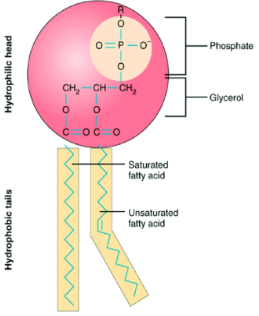
\includegraphics[width=0.35\textwidth,height=7cm]{membrane.png}}
  \caption{membrane subunit}
\end{figure}



\noindent it. The head is connected to the tails through a small backbone, so the whole molecule looks kind of like a matchstick or a two-tailed kite. Because one part of the molecule wants to be near water and the other part wants to avoid it, phospholipids naturally arrange themselves into layers when they’re in water. These layers form flexible membranes that act a lot like soft polymer sheets—they can bend, move, and even stretch a little. In fact, scientists often use ideas from polymer physics to study how these membranes behave, especially when trying to understand things like how viruses wrap themselves up or how they enter cells.


\subsection*{III. Genome/DNA/RNA}
DNA and RNA are long chains made up of smaller units called nucleotides. Each nucleotide is like a puzzle piece, made of a sugar, a phosphate group, and a nitrogen base. In DNA, the sugar is called deoxyribose, and in RNA, it’s ribose. The bases are the parts that carry genetic 

\begin{figure}[!ht]
  \centering
  
   \fbox{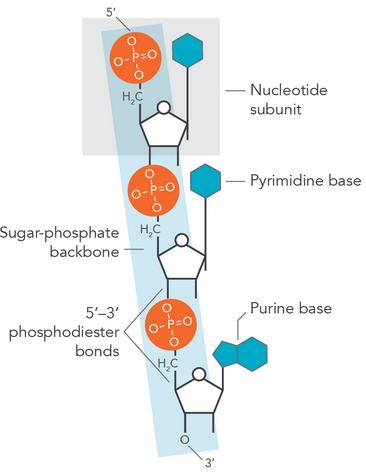
\includegraphics[width=0.35\textwidth,height=8cm]{genome.png}}

  \caption{Nucletide subunits}
\end{figure}


\noindent information—A, T, G, and C in DNA, and A, U, G, and C in RNA (with U replacing T in RNA). These nucleotides link together through bonds between the phosphate of one and the sugar of the next, forming a backbone, kind of like beads on a string. 





Nucleotides, the building blocks of RNA and DNA, act as repeating units  that form larger macromolecules, similar to how polymers are made from repeating monomers. The polymeric nature allows genomic material to adopt different shapes and configurations. Just as polymers can interact with other compounds, RNA and DNA can form secondary structures and interact with proteins, which is essential for processes like gene expression and viral assembly. Polymers can have various structures—linear, branched, or crosslinked—allowing them to be flexible, adaptable, and capable of forming diverse shapes and configurations.  DNA and RNA are biopolymers, and it means they have a polymeric nature that enables them to fold, coil, and interact with other molecules based on factors like sequence, chemical interactions, and environmental conditions.



This makes DNA and RNA behave like polymers—long, repeating chains that can twist, bend, and fold. DNA usually forms a double helix, with two strands held together by base pairing (A with T, and G with C), while RNA is usually single-stranded and folds into all kinds of shapes. In science, especially in physics, we can think of DNA and RNA as flexible polymers, which helps us understand how they fold up inside tiny spaces—like the inside of a virus.

\begin{figure}[!ht]
  \centering
   \fbox{\includegraphics[width=0.45\textwidth,height=4cm]{chromatin.png}}
  
  %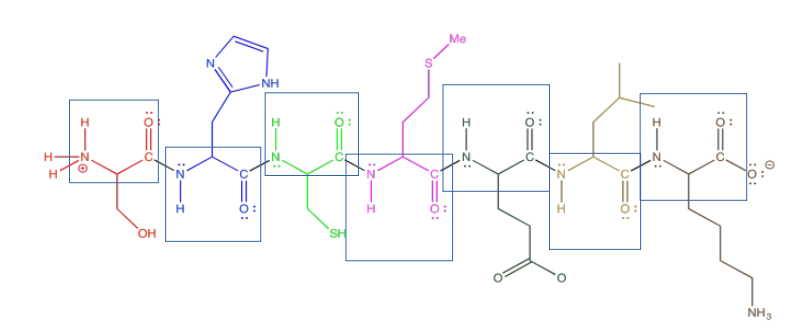
\includegraphics[width=0.3\textwidth,height=4cm]{protein.png}  % Adjust width or height as needed
  \caption{DNA, Chromatin and Chromosome\cite{byjus_chromatin}}
\end{figure}




\subsection*{IV. Protein/Amino Acid chain}
Proteins are natural polymers made up of amino acids, which are like the individual links in a chain. Each amino acid has the same basic structure: a central carbon atom (called the alpha carbon) bonded to a hydrogen, an amino group (–NH$_2$), a carboxyl group (–COOH), and a unique side chain, known as the R group. These amino acids connect through peptide bonds, forming a 

\begin{figure}[!ht]
  \centering
   \fbox{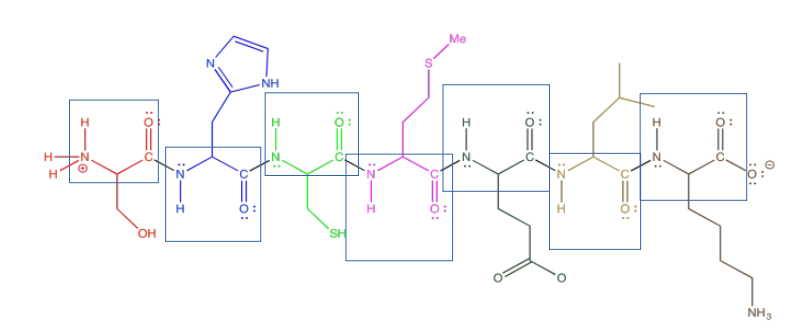
\includegraphics[width=0.5\textwidth,height=4cm]{protein.png}}
  
  %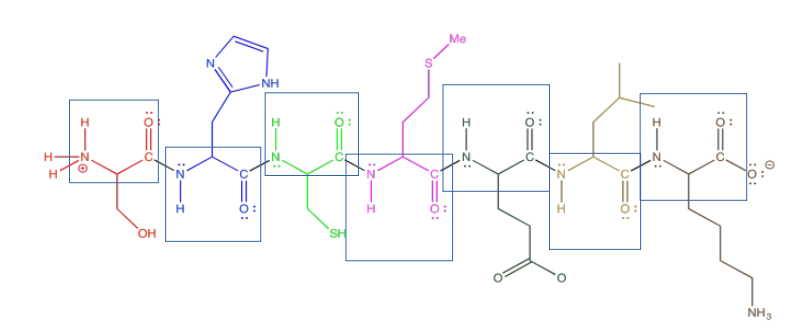
\includegraphics[width=0.5\textwidth,height=4cm]{protein.png}  % Adjust width or height as needed
  \caption{Amino acid chain}
\end{figure}

A protein is fundamentally a polymer—a long chain of amino acids linked together. In its unfolded state, this chain behaves like a typical polymer: flexible, disordered, and dynamic. As it folds, however, it transforms into a highly organized and functional structure. The folding process begins with the formation of local secondary structures, such as alpha helices and beta sheets, followed by the overall folding of the chain into a specific three-dimensional shape (tertiary structure). In some cases, multiple folded chains assemble into a larger complex, forming a quaternary structure. Despite this transformation, the polymer backbone remains; it’s simply arranged in a compact and functional form.

Once folded, a protein may not resemble a simple polymer visually or functionally. Though still composed of repeating amino acid units, these units are now intricately arranged—spiraling into helices, flattening into sheets, and looping into turns that define the protein's function. It no longer appears as a linear chain, but it retains key polymer-like properties: flexibility, responsiveness, and dynamic movement in response to its environment.

This underlying polymer nature is why coarse-grained (CG) modeling remains effective, even for folded proteins. Rather than representing every atom, CG models group atoms into larger units or “beads,” allowing us to study large-scale behaviors—such as folding, conformational changes, or molecular interactions—without the computational cost of atomic detail. Because proteins are still polymers at their core, coarse-graining offers a powerful way to explore their structure and function at a broader scale.


\begin{figure}[!ht]
  \centering
   \fbox{\includegraphics[width=0.5\textwidth,height=6cm]{complex.protein.png}}
  
  %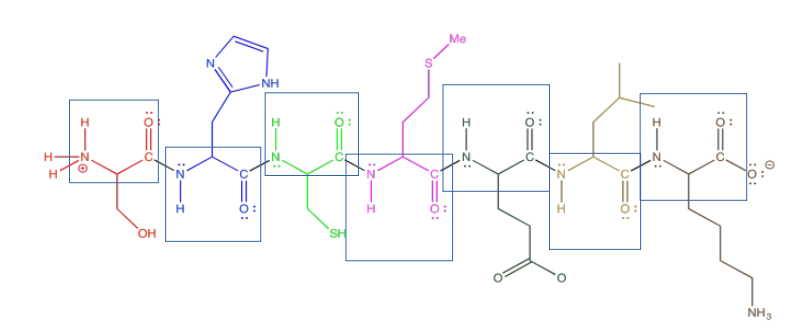
\includegraphics[width=0.5\textwidth,height=4cm]{protein.png}  % Adjust width or height as needed
  \caption{Protein}
\end{figure}






\section*{History of Coase grained models }

Back in the 1960s and 70s—long before computational biology became mainstream—polymer scientists were already coming up with clever ways to simplify and understand how long-chain molecules behave. They built theoretical models like the freely-jointed chain, worm-like chain, and Gaussian chain, each designed to capture how flexible or stiff a polymer might be, and how it moves in space. These early ideas laid the foundation for what we now call coarse-grained simulations. Around the same time, the bead-spring model came into play — a simple but powerful way to represent a polymer as a series of connected beads linked by springs. It turned out to be incredibly useful for studying how polymers move, tangle, and interact in bulk materials — and remarkably, this same basic idea is still widely used today in modern polymer simulations.\\

Coarse-grained modeling started making an impact in protein science back in the 1970s, when researchers like Michael Levitt, Ariel Warshel, and Martin Karplus began simplifying protein structures to make them easier to study. Instead of modeling every single atom, they used a more abstract approach—sometimes representing entire amino acids as single "beads." This allowed scientists to simulate complex processes like protein folding and movement, which would have been far too computationally demanding with full atomic detail at the time. As the field evolved, so did the models. The Go model, for example, focused on capturing the folded shape of proteins in a minimalistic way, while more advanced structure-based models helped researchers understand folding pathways, domain motion, and protein aggregation. In the 2000s, the MARTINI force field took things even further, allowing proteins to be simulated in realistic environments like cell membranes and solvents. Thanks to these developments, scientists can now explore protein dynamics and interactions on scales that were once unimaginable.\\

Coarse-grained models found a natural fit in the study of lipid membranes in the early 2000s, when researchers began adapting these techniques to simulate the complex behavior of biological membranes. A major breakthrough came with the development of the MARTINI model, which represented lipids and solvents using just a few beads per molecule—typically three to four. This simplification made it possible to simulate large-scale membrane systems, including lipid bilayers, fusion events, and phase separation, all over timescales far beyond what atomistic models could handle. Scientists could now study how membrane proteins insert, move, and interact within lipid environments, as well as dynamic processes like vesicle formation, pore opening, and even viral fusion with host cells. Coarse-grained modeling also enabled the simulation of entire organelles or membrane-associated complexes that would be computationally unmanageable in full atomic detail, opening up new possibilities for understanding the structure and function of cellular membranes.\\

Coarse-grained modeling has become a vital tool for understanding how our genomes are organized and function at a large scale. Instead of trying to simulate every atom in a DNA molecule — an impossible task given that chromosomes span millions or even billions of base pairs — researchers started simplifying the problem in smart ways. Since the mid-2000s, with advances in computational power and experimental methods, researchers began modeling DNA and chromatin using coarse-grained approaches that strip away unnecessary atomic detail while keeping the essential features.

One popular method is the “bead-on-a-string” model, where each bead represents a segment of DNA or a nucleosome. These models, rooted in polymer physics, let researchers explore how DNA folds, forms loops, and compacts into the crowded space of the nucleus. Over the past decade, such models have helped understand the the folding of genome inside interpahse nulcei \cite{Lizana2024}.\\




By focusing on the big picture, coarse-grained modeling gives us a way to study the genome not just as a long string of genetic code, but as a dynamic and functional 3D structure — one that plays a critical role in how cells behave and how genes are regulated. In this research, We study how the genome and the membrane undergo shape changes and fluctuations over time.



\section*{Method} 
\subsection*{1 Models}
\subsection*{1.1 Coase-grain models}

\subsection*{1.1.1 Adveantage of Coase-grain model}



	Using a coarse-grain model in polymer science is really helpful because it makes things simpler and more efficient, especially when dealing with large and complex systems. One of the biggest reasons to use coarse-graining is that it saves a lot of computational power. Polymers are often made up of thousands or even millions of atoms, so simulating each individual atom takes a huge amount of time and resources. Instead of modeling each atom, a coarse-grain model groups several atoms or monomers into a "bead," which reduces the number of particles in the simulation. This allows researchers to study bigger systems and longer timescales without overwhelming their computers.

	Another advantage is that coarse-graining allows us to focus on the big picture of polymer behavior. At the atomic level, polymers have tons of detailed interactions, but often what we care about are the overall properties, like how the polymer stretches, bends, or reacts to forces. Coarse-graining simplifies this by letting researchers study these larger-scale behaviors without getting caught up in the tiny atomic details, which are often less important for understanding real-world polymer behavior.
	
	Coarse-grain models also make it easier to model interactions between polymers. Instead of focusing on each individual monomer, coarse-graining represents groups of monomers as beads. This makes the interactions between polymer chains less complex and easier to study. This is really useful for studying complicated systems like polymer networks, gels, or blends, which would be too difficult to model atom by atom.\\
	
	
	Another reason coarse-grain models are so valuable is that they help rus simulate larger systems over longer periods of time. By reducing the number of particles in the model, simulations can run much faster and allow for studies over longer timescales. Instead of simulating each tiny atom’s movement, which can take a long time, coarse-graining lets researchers study the overall behavior of the polymer chain over much longer periods. This is really useful for looking at things like polymerization processes or phase transitions that occur over time.
	
	Coarse-grain models also focuses on the important polymer properties that matter most, like flexibility, shape changes, and how polymers self-assemble. These properties are often determined by the overall structure of the polymer, not by the exact positions of every single atom. So by simplifying the model, researchers can study how polymers fold, how they form membranes, or how they interact with other molecules, without having to get into the atomic-level details.\\
	
	Finally, coarse-grain models are essential for designing new materials. When researchers are developing new types of polymers—whether for drug delivery, biodegradable plastics, or high-performance materials, these models help predict how the polymer will behave in different environments. This helps researchers optimize the materials for real-world uses without needing to simulate every tiny detail.
	In the end, coarse-grain models are incredibly useful in polymer science because they simplify complex systems, making it easier to study their behavior. They save time and computational power while still allowing scientists to focus on the big picture—like how polymers stretch, bend, and interact—helping to design better materials and understand how polymers work in the real world.
	



\subsection*{1.1.2 Assumption of Coarse grain model}
Coarse-grained models come with several assumptions that are critical for their application:\\
    1. Homogeneity:\\
    It is often assumed that the system is uniform, meaning properties do not vary significantly across space. \\
    2. Bead Representation:\\
        Each bead represents a group of atoms, assuming they behave as a single entity in terms of interactions, which may not always reflect the nuances of molecular behavior. \\
    3. Simplified Interactions:\\
        The models typically ignore specific interactions at the atomic level, such as hydrogen bonding or van der Waals forces, unless they are effective at the coarse-grained level. \\
    4. Mean-Field Approximations:\\
        Coarse-grained models often use mean-field approximations, averaging the effects of all other particles on any given particle, simplifying the interactions that can be complex in real systems. \\
    5. Fixed Connectivity:\\
        In polymer applications, it usually assumes fixed connectivity between beads, which may not fully account for the flexibility in the actual polymer chains. \\ 

\subsection*{1.2 Excluded volume}

Excluded volume is an essential aspect of coarse$-$grained (CG) modeling, ensuring that two particles do not occupy the same space. Without it, particles in a simulation may overlap or penetrate each other, leading to unphysical results. To account for excluded volume, repulsive interaction potentials—such as the Lennard-Jones potential or its softer variants used in models like MARTINI or DPD—are applied. These potentials create a repulsive force that prevents particles from getting too close. Key parameters like bead size ($\sigma$) and interaction strength ($\varepsilon$) must be carefully tuned to reflect the physical size and behavior of the particles.

Before running a simulation, energy minimization and equilibration steps are typically used to eliminate any initial overlaps and ensure a stable starting configuration. Additionally, the mapping of atoms to CG beads should be realistic; inaccurate mappings can distort how particles pack and interact. Properly enforcing excluded volume is particularly important in biomolecular and polymer systems, where structural integrity and thermodynamic behavior depend on realistic spatial constraints. Ignoring or mishandling excluded volume can compromise the accuracy and reliability of the simulation.



\subsection*{1.3 Kremer-Grest Model for DNA chain}

	
The Kremer-Grest (KG) model is a bead-spring type of coarse-grained model. KG model is specifically for polymers,including those relevant to chromosome structure and genome organization, and a popular way to simulate polymers in computer-based molecular dynamics. It is a specific, well-defined bead-spring model that includes Lennard-Jones (LJ) potential for excluded volume (non-bonded interactions) and FENE (Finitely Extensible Nonlinear Elastic) potential for the bonds between adjacent beads.	


Instead of tracking every atom, it simplifies the system by representing each polymer chain as a string of connected beads. These beads interact with each other in two main ways: non-bonded beads repel each other using something called the Lennard-Jones (LJ) potential, which helps prevent them from overlapping, and bonded beads (those directly connected in the chain) are held together by a FENE spring, which stretches like a real polymer bond but can't break or stretch too far. To keep the system at a steady temperature—like it would be in a real fluid—a Langevin thermostat is often used, adding both friction and random kicks to the beads. The model is simple, efficient, and captures the large-scale behavior of polymers really well, which is why it's used so widely in polymer research.	
	

Kresmer$-$grest Model is more physically realistic for polymers than a basic harmonic model and bead$-$spring model.
It prevents bond crossing (thanks to FENE + LJ) and it has been extensively validated and used in thousands of studies.

\begin{figure}[!ht]
  \centering
  \fbox{\includegraphics[width=0.25\textwidth,height=4cm]{beadspring.png} }
  \caption{Bead-Spring Representation of a Polymer Chain (Kremer–Grest Model)}
\end{figure}


\begin{itemize}
  \item \textbf{FENE spring:} \( k = 30 \), \( R_0 = 1.5 \)
  \item \textbf{Lennard-Jones (LJ) potential:} \( \varepsilon = 1 \), \( \sigma = 1 \), cutoff \( r_c = 2^{1/6} \sigma \)
  \item \textbf{Time integration (Langevin thermostat):} friction \( \gamma = 0.5 \), temperature \( T = 1.0 \)
\end{itemize}


\subsection*{1.4 Simple liquid Models for the organelles surrounding DNA}

Simple liquid models that help understand the structure and behavior of polymer fluids in crowded environments. Specifically, the simple liquid models referenced include Hard Sphere Model and Lennard-Jones Model. 


Hard sphere model is used to understand the behavior of particles in crowded environments, where the excluded volume effect becomes important. 


The Lennard-Jones model accounts for both attractive and repulsive forces between particles, which is important in understanding the interactions within fluids and condensed matter. It helps model the behavior of molecules, especially in non-ideal conditions like those found in crowded environments. 

\subsection*{1.5 Helfrich-Canham Model for the membrane}

The Helfrich-Canham model, a specific type of continuum model, focuses on the membrane's curvature elasticity and bending energy\cite{Bassereau2014}.
\begin{figure}[!ht]
  \centering
  \includegraphics[width=0.45\textwidth,height=4cm]{fobinacci.network.png} 
  \caption{Left image: Fiboncci model  Right image: }
\end{figure}

Continuum models are a powerful framework used to describe and simulate the large-scale, smooth behavior of biological membranes (and other materials) without tracking individual atoms or molecules. Instead of focusing on discrete particles like in molecular dynamics, continuum models treat the membrane as a continuous surface or material with defined physical properties.

To model the membrane, we start by creating a triangular mesh, which breaks the curved surface into flat triangles. This mesh should form a closed shape, like a sphere, to represent structures such as vesicles. Each triangle has corners called vertices, and each vertex has a position in 3D space. This setup makes it possible to calculate important properties like curvature and surface area, which are needed to compute the membrane’s bending energy. You can build this mesh using Python tools like trimesh or vedo, or by writing your own code to create an icosphere—a sphere made by dividing an icosahedron into smaller triangles. This mesh gives you the base needed to apply the Helfrich-Canham model in your simulations.

To model the genome, make a chain of beads, each one representing a segment of the genome. Each bead has a 3D position, and the list looks like: beads = [b1, b2, ..., bn]. Connect each bead to its neighbor with a spring, which keeps the distance between them close to a set value. You can use a harmonic potential or FENE potential to describe the spring force. The spring energy is:






Also, include excluded volume so beads don’t overlap. You can do this using a soft repulsive force, like a Lennard-Jones potential.


To simulate a genome inside a lipid membrane, we need to make sure the genome stays inside and doesn’t leave the membrane. This is done by adding a boundary constraint. One simple method is a hard-wall constraint, which blocks any genome bead from moving outside the membrane by rejecting such moves. Another method is to use a soft repulsive potential, like the Lennard-Jones force, which gently pushes beads back when they get too close to the membrane boundary. These methods keep the genome inside the membrane while still letting it move and fluctuate naturally.


 
 
 
 
  After that, we define a cutoff distance—a threshold that determines whether two beads are close enough to be connected. For each pair of beads, we calculate the distance between them, and if it’s less than or equal to the cutoff, we connect them with a virtual spring. These springs represent interactions or flexibility between the nodes. 
  
	Once all the connections are made, we construct what's called the Kirchhoff matrix (or the GNM matrix). In this matrix, a value of -1 is placed at the off-diagonal positions where two beads are connected, and 0 where they're not. The diagonal entries are set so that each row adds up to zero, which simply reflects how many connections each bead has. This matrix is the core of the GNM approach—it captures the structure of the network and can be used to study how the system might flex, shift, or vibrate as a whole. By following these steps, you turn a static arrangement of beads on a sphere into a dynamic network model that can simulate real-world molecular or physical behaviors.












\subsection*{1.6 Summary of the models}
Coarse-grain model and simple liquid models are valuable tools in understanding how particles interact in condensed matter systems, such as polymer fluids, from both an energetic (energy of interactions) and entropic (disorder and randomness) perspective.


\subsection*{II.Simulation}


\subsection*{1.1 Monto Carlo simulation}

Monte Carlo (MC) simulation is a technique used to explore different configurations of a system by randomly sampling possible states, based on probability rules that often relate to energy. Instead of following every tiny movement of particles over time—like molecular dynamics does—Monte Carlo takes a different approach. It “jumps” from one possible state to another and decides whether to accept or reject each move depending on how favorable it is, typically using criteria like energy minimization.
This method becomes especially powerful when combined with coarse-grain (CG) models. Coarse-graining simplifies complex systems by grouping atoms or monomers into larger units, reducing the number of particles and interactions. This makes the system easier and faster to simulate, which is perfect for Monte Carlo techniques. With fewer variables to track, MC simulations can explore a much wider range of configurations in less time.
Using MC with CG models is particularly useful for studying large-scale behaviors like polymer folding, self-assembly, phase transitions, or how polymers interact with other surfaces or structures. Since you don’t need to worry about every atomic detail, you can focus on understanding the broader behavior of the material. For instance, in a coarse-grain polymer simulation, MC methods might rotate parts of the polymer chain, stretch or shift segments, or rearrange them—checking each time how these changes affect the system’s overall energy or structure.
In short, Monte Carlo simulations and coarse-grain modeling work hand in hand. Together, they make it possible to study complex polymer systems more efficiently and gain insights that would be hard to reach using more detailed, atomistic approaches.

\subsection*{1.2 Assumpations of Monto Carlo simulation}


    1. Randomness is representative
    
The simulation assumes that the random inputs it uses (often generated using pseudo-random number generators) adequately represent the variability and uncertainty of real-life scenarios.\\

\noindent 2. Independent trials
    
Each simulation run (or trial) is assumed to be independent of the others. The outcome of one run does not affect the outcome of another.

\noindent    3. Known probability distributions
    
The input variables must follow known probability distributions (e.g., normal, uniform, triangular, etc.). The accuracy of the results relies heavily on how well these distributions reflect real-world behavior.

\noindent  4. Large number of iterations
    
The law of large numbers is a key assumption — with a large enough number of trials, the average of the simulated outcomes should approximate the expected value. More iterations generally improve accuracy.

\noindent5. System/process remains stable
    
The simulation assumes that the underlying process or system doesn’t change over time during the simulation (i.e., it's stationary).

\noindent    6. Model structure is correct

The simulation is only as good as the model it's based on. It assumes the mathematical or logical structure you build reflects the real-world process correctly.


We simplify the genome$-$membrane system using a coarse-grained model,and use Monte Carlo simulation to explore its behavior of the system. Monte Carlo can help fit the parameters of a coarse-grained model.Coarse-grained models and Monto carlo simulate large, complex systems (like polymers, membranes) efficiently and with reasonable accuracy.




\subsection*{III. Summary}
Viral genomes (like those in Monkeypox and SARS-CoV-2) behave similarly to a polymer chain packed inside a small, crowded space (the viral capsid/membrane). The project aims to extend existing models and Monto Carlo simulation to study how the genome's architecture (shape, length, and flexibility) affects the overall shape of a virus. This will help us understand how viral genomes and membranes interact, which is crucial for predicting viral structures and behavior.



\subsection*{Formular}

%\frac{V(r)}{k_B T} = -\Gamma \frac{\exp(-\kappa_1 r)}{r} +V
\begin{equation}
E(r) = -\Gamma \frac{\exp(-\kappa_1 r)}{r} K_B T\cite{yukawa1935} +V
\end{equation}

The Yukawa potential V(r) describes how two particles interact when their force has a finite range

E(r) potential energy as a function of distance r\\
\(\Gamma\) is the interaction strength,\\
\(\kappa_1\) is the screening parameter \\
\(r\) is the distance, \\
Negative sign (-) indicates the interaction is attractive.\\
The left-hand side \( \frac{V(r)}{k_B T} \) indicates how strong the interaction is compared to the typical thermal energy \( k_B T \).\\

The potential is negative (\( -\Gamma \)), meaning it is attractive — it tends to pull particles together.

\noindent The form \( \frac{e^{-\kappa_1 r}}{r} \) means:

\begin{itemize}
    \item At short distances (\( r \to 0 \)), the potential behaves like \( \sim \frac{1}{r} \) — like a Coulomb (electrostatic) potential.
    \item At large distances (\( r \to \infty \)), the potential decays exponentially because of the \( e^{-\kappa_1 r} \) — it becomes very small quickly.
    \item \( \kappa_1 \) controls how short-ranged the potential is: larger \( \kappa_1 \) means the force dies off quicker.
\end{itemize}



\begin{equation}
V= \int \left( \frac{\kappa_2}{2} (C_1 + C_2 - C_0)^2 + \sigma \right) dA
\end{equation}


Total Energy of the Bead-Spring Genome:

\begin{equation}
E_{\text{total}} = E_{\text{spring}} + E_{\text{LJ}}
\end{equation}


\begin{equation}
E_{\text{spring}} = \sum_{i=1}^{N-1} \frac{k}{2} \left( \left| \vec{r}_{i+1} - \vec{r}_i \right| - l_0 \right)^2
\end{equation}


\begin{equation}
E_{\text{LJ}} = \sum_{i=1}^{N} \sum_{j=i+2}^{N} 4\varepsilon \left[ \left( \frac{\sigma}{r_{ij}} \right)^{12} - \left( \frac{\sigma}{r_{ij}} \right)^6 \right]
\end{equation}

A coarse-grained model simplifies molecules by grouping atoms into beads but still retains discrete particles and molecular interactions.

A continuum membrane model goes further—it treats the membrane as a continuous, deformable surface, governed by elasticity theory rather than particle-based forces.

while continuum models are not considered the classical coarse-grained, they are part of the same multiscale modeling, but just at a larger, more abstract scale.

Most notably the Helfrich-Canham model, which defines the bending energy of the membrane as:
\begin{equation}
E = \int \left( 2\kappa (2H - C_0)^2 + \bar{\kappa} K \right) \, dA
\end{equation}





The Helfrich–Canham model, a specific type of continuum models, focuses mainly on bending energy and curvature-driven deformations, It describes the total energy of a membrane by combining two main contributions: bending energy and surface tension energy. The bending energy reflects how much the membrane curves away from its preferred, or spontaneous, shape. Meanwhile, the surface tension energy accounts for the cost of stretching the membrane — it increases when the membrane's surface area grows. Together, these terms help explain how membranes bend, stretch, and maintain their shape in different environments.


The total free energy of a closed lipid bilayer:
Continuum Form (Analytical Model):

\begin{equation}
E = \int_{\text{membrane}} \left[ 2\kappa (2H - C_0)^2 + \bar{\kappa} K \right] \, dA + \lambda A + PV
\end{equation}
\begin{align*}
\kappa &:\ \text{bending rigidity} \\
\bar{\kappa} &:\ \text{Gaussian modulus} \\
H &:\ \text{mean curvature} \\
K &:\ \text{Gaussian curvature} \\
C_0 &:\ \text{spontaneous curvature} \\
A &:\ \text{total surface area} \\
\lambda &:\ \text{Lagrange multiplier for area constraint (surface tension)} \\
P &:\ \text{Lagrange multiplier for volume constraint (pressure)}\\
V &:\ \text{enclosed volume} 
\end{align*}

It models the elastic energy of a smooth, flexible surface (like a lipid bilayer vesicle) as a function of curvature. This model alone does not specify how lipids or proteins are distributed on the surface — it just tells you what shapes minimize bending energy.






\begin{equation}
\begin{split}
F_b^{\text{discrete}} &= \frac{1}{2} \tilde{\kappa} \sum_{\langle \alpha, \beta \rangle} \left| \mathbf{n}_\alpha - \mathbf{n}_\beta \right|^2 \\
&= \tilde{\kappa} \sum_{\langle \alpha, \beta \rangle} \left( 1 - \mathbf{n}_\alpha \cdot \mathbf{n}_\beta \right) 
\end{split}
\end{equation}







The form sums over pairs of adjacent faces \(\langle \alpha, \beta \rangle\).

\begin{itemize}
    \item \(\mathbf{n}_\alpha\) and \(\mathbf{n}_\beta\) are unit normals to the faces.
    \item \(\mathbf{n}_\alpha \cdot \mathbf{n}_\beta = \cos \theta\), where \(\theta\) is the angle between adjacent normals.
    \item \(\tilde{\kappa}\) is an effective bending modulus (often different from \(\kappa\)).
\end{itemize}


The Discrete Bending Energy (Angle-based Form)
\begin{equation}
E_{\text{mem}} = \kappa \sum_{\text{edges } e} \left(1 - \cos \theta_e \right)\cite{gompper1997triangulated}
\end{equation}

This is a discretized approximation of the bending energy, suitable for numerical simulations Monte Carlo or molecular dynamics. It captures curvature using local triangle normals instead of differential geometry.

Area constraint
\begin{equation}
E_{\text{area}} = \lambda(A - A_0)^2
\end{equation}

Volume constraint:
\begin{equation}
E_{\text{Volume}} = \lambda(V - V_0)^2
\end{equation}



\begin{equation}
\Delta E = (E_{\text{membrane}}^{\text{new}} + E_{\text{polymer}}^{\text{new}}) - (E_{\text{membrane}}^{\text{old}} + E_{\text{polymer}}^{\text{old}})
\end{equation}


Metropolis rule:

\begin{equation}
P = \min\left(1, \exp\left(-\frac{\Delta E}{k_B T}\right)\right)
\end{equation}

If move is accepted then positions will be updated. If rejected then the move will be reverted.

Simulating realistic physical conditions, since many experiments happen at constant pressure (example:1 atm) and temperature  (example: 298 K).

\noindent NPT Ensemble (Isothermal–Isobaric Ensemble)

NPT stands for:

    N = Number of particles (constant)

    P = Pressure (constant)

    T = Temperature (constant)
    
    Under NPT conditions, the system’s pressure is controlled, allowing the volume to change naturally over time. In one approach, the membrane is initialized with a fixed oval or ellipsoidal shape, defined by the input parameters a, b, and c, which represent the lengths along its three principal axes. These parameters remain constant during the simulation, so the membrane maintains its overall shape while still allowing local fluctuations and interactions with the genome inside.

In another approach, the parameters a, b, and c are allowed to fluctuate during the simulation. This means the membrane can expand, shrink, or reshape dynamically in response to internal forces exerted by the genome. Such flexibility promotes more realistic interactions between the genome and the membrane — for example, the genome may push outward and deform the membrane, while changes in membrane tension or curvature can influence how the genome is organized. Using NPT conditions in this way provides a natural and dynamic view of the interplay between membranes and genomes in biological systems.

\noindent NVT Ensemble (Canonical Ensemble)

NVT stands for:

    N = Number of particles (constant)

    V = Volume (constant)

    T = Temperature (constant)

Under NVT conditions, the volume of the system is fixed, meaning the membrane is constrained and cannot expand or contract. In one approach, the membrane is initialized with an oval or ellipsoidal shape, defined by input parameters a, b, and c, representing the lengths along its three principal axes. These parameters remain constant throughout the simulation, so the membrane keeps its shape even as the genome inside moves or grows. Because the membrane cannot adapt naturally to changes, any pressure exerted by the genome builds up inside, sometimes leading to artificial forces that would not normally appear in a flexible system.

In another approach, even though the overall volume remains fixed under NVT, small local fluctuations in the shape of the membrane are allowed while still keeping a, b, and c centered around their initial values. In this case, the membrane can slightly deform in response to internal forces from the genome without changing its total volume. While the confinement effect is still strong, allowing limited local fluctuations provides a somewhat more realistic interaction between the genome and the membrane. Studying the membrane–genome relationship in either method under NVT is useful for early-stage stabilization or when specifically exploring how genomes behave in confined, rigid environments.



The genome of the Monkeypox virus is a double-stranded DNA, approximately 190 kb (kilobases) in length, which equals about 95 kbp (kilobase pairs). This genomic length corresponds to a substantial contour length of approximately 3000 nm. This indicates that the genetic material is significantly longer than the physical dimensions of the virus itself, which measures around 250 nm long. 
These viral particles can display spherical and oval shapes, indicating different developmental stages: immature virions tend to be spherical, while mature virions adopt an oval shape. This morphological differentiation can be important for recognizing stages in the virus life cycle and understanding how these changes may affect infectivity. The transition from spherical to oval shapes may be linked to the maturation process, influencing the virus's ability to enter host cells and replicate effectively.\\

The shape of viral particles, like those seen in the Monkeypox virus, can reveal a lot about what stage they’re at in their life cycle. In the early phases, the virus forms immature virions that are usually spherical. This round shape isn’t random—it helps the virus begin assembling its genetic material and proteins in a flexible, efficient way. At this point, the virus is just starting to come together, packaging its core components. As it matures, the virus goes through structural 

\begin{figure}[!ht]
  \centering
  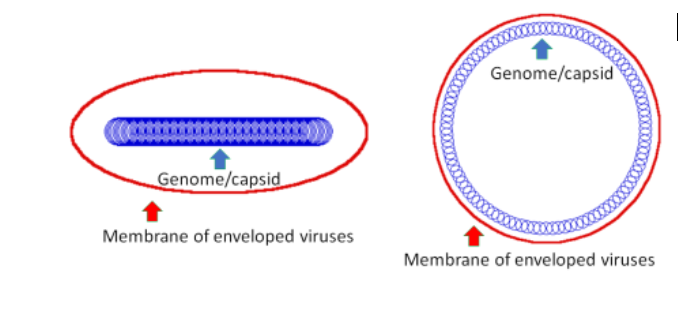
\includegraphics[width=0.5\textwidth,height=4cm]{monkeypox.png}  % Adjust width or height as needed
  \caption{Preliminary 2D model studies to
investigate the effect of the geometry of a
genome on the shape of a virus. A rod-like
genome induces an elliptic shape whereas a
circular genome leads to a circular shape.}
\end{figure}

\noindent changes that shift its shape from spherical to oval. This transformation involves the rearrangement of viral proteins, which makes the particle more stable. The oval shape not only helps the mature virion survive better outside the host but also improves its ability to attach to and enter host cells. This increased stability and better interaction with host cell receptors make the mature, oval-shaped virus more infectious and better equipped to replicate once inside a host.




We begin by modeling the phage DNA as a fine-grained polymer, such as a worm-like chain, which accurately represents the stiffness and bending behavior of real double-stranded DNA. This model is placed within a confined volume that mimics the $60\,\text{nm} \times 150\,\text{nm}$ prolate icosahedral capsid of phage $\lambda$.
 


Next, we simulate stepwise DNA packaging by applying a force from a virtual packaging motor that mimics the biological motor’s function. At each step, a small segment of DNA is inserted into the capsid, and we calculate the energy required to overcome internal forces such as electrostatic repulsion and bending stress. This allows us to track the buildup of internal pressure as the capsid fills, which can then be directly compared to experimentally measured force-extension (packing) curves from optical tweezer studies.

Once the genome is fully packaged, we simulate ejection dynamics by triggering a release mechanism, such as opening a virtual portal in the capsid. The DNA is then allowed to eject, and we record the ejection speed, force, and time as the internal pressure drives the genome out. These simulation results can be compared to experimental data from ejection assays and osmotic suppression experiments, where external osmotic agents slow or block ejection and allow researchers to measure the pressure driving it.


By tuning simulation parameters (e.g., DNA stiffness, packing force, ionic strength) and validating against high-quality experimental datasets from phage $\lambda$, we ensure that our model reproduces the biological and physical behavior observed in the lab. In bacteriophages, the DNA experiences strong forces—up to around 60 picoNewtons—during the packaging and ejection process. These forces mainly come from the bending stiffness of the DNA and the repulsion between tightly packed strands. Experiments using osmotic suppression have shown that it's possible to stop DNA ejection by applying external PEG solutions that create about 20 to 40 atmospheres of pressure\cite{Grayson2006}.




\end{flushleft}
\bibliographystyle{unsrt}
\bibliography {references}  

\end{document}




